\RequirePackage{pdfmanagement-testphase}
\DeclareDocumentMetadata {lang=en-US}

% xmp metadata for pdf
% Originally used \usepackage[a-2a]{pdfx}
% \usepackage{hyperxmp} replaced it
% \RequirePackage{pdfmanagement-testphase} replaced it
% \PassOptionsToPackage{enable-debug,check-declarations}{expl3} broke with version 0.9 of tagpdf
% \ExplSyntaxOn no need for these 3 lines because metadata can handle it
% \pdfmanagement_add:nnn{Catalog}{Lang}{(enUS)} enUS is wrong, should be en-US
% \ExplSyntaxOff

\documentclass[11pt,
  english,
  a4paper,
]{article}
\usepackage{sa4ss}
\usepackage{amsmath,amssymb,array}
\usepackage{booktabs}

% From tagged-template.latex
\usepackage{lmodern}
\usepackage{ifxetex,ifluatex}
\ifnum 0\ifxetex 1\fi\ifluatex 1\fi=0 % if pdftex
  \usepackage[T1]{fontenc}
  \usepackage[utf8]{inputenc}
  \usepackage{textcomp} % provide euro and other symbols
\else % if luatex or xetex
  \usepackage{unicode-math}
  \defaultfontfeatures{Scale=MatchLowercase}
  \defaultfontfeatures[\rmfamily]{Ligatures=TeX,Scale=1}
\fi

% Use upquote if available, for straight quotes in verbatim environments
\IfFileExists{upquote.sty}{\usepackage{upquote}}{}
\IfFileExists{microtype.sty}{% use microtype if available
  \usepackage[]{microtype}
  \UseMicrotypeSet[protrusion]{basicmath} % disable protrusion for tt fonts
}{}
\makeatletter
\@ifundefined{KOMAClassName}{% if non-KOMA class
  \IfFileExists{parskip.sty}{%
    \usepackage{parskip}
  }{% else
    \setlength{\parindent}{0pt}
    \setlength{\parskip}{6pt plus 2pt minus 1pt}}
}{% if KOMA class
  \KOMAoptions{parskip=half}}
\makeatother
\usepackage{xcolor}
\IfFileExists{xurl.sty}{\usepackage{xurl}}{} % add URL line breaks if available
\hypersetup{
  pdftitle={Evaluating available information to determine stock management delineation for copper rockfish (Sebastes caurinus) off the U.S. West Coast},
  pdflang={en},
  hidelinks,
  pdfcreator={LaTeX via pandoc}}
\urlstyle{same} % disable monospaced font for URLs
\usepackage{longtable}
% Correct order of tables after \paragraph or \subparagraph
\usepackage{etoolbox}
\makeatletter
\patchcmd\longtable{\par}{\if@noskipsec\mbox{}\fi\par}{}{}
\makeatother
% Allow footnotes in longtable head/foot
\IfFileExists{footnotehyper.sty}{\usepackage{footnotehyper}}{\usepackage{footnote}}
\makesavenoteenv{longtable}
\usepackage{graphicx}
\makeatletter
\def\maxwidth{\ifdim\Gin@nat@width>\linewidth\linewidth\else\Gin@nat@width\fi}
\def\maxheight{\ifdim\Gin@nat@height>\textheight\textheight\else\Gin@nat@height\fi}
\makeatother
% Scale images if necessary, so that they will not overflow the page
% margins by default, and it is still possible to overwrite the defaults
% using explicit options in \includegraphics[width, height, ...]{}
\setkeys{Gin}{width=\maxwidth,height=\maxheight,keepaspectratio}
% Set default figure placement to htbp
\makeatletter
\def\fps@figure{htbp}
\makeatother
\setlength{\emergencystretch}{3em} % prevent overfull lines
\providecommand{\tightlist}{%
  \setlength{\itemsep}{0pt}\setlength{\parskip}{0pt}}
\setcounter{secnumdepth}{5}
\ifxetex
  % Load polyglossia as late as possible: uses bidi with RTL langages (e.g. Hebrew, Arabic)
  \usepackage{polyglossia}
  \setmainlanguage[]{english}
\else
  \usepackage[shorthands=off,main=english]{babel}
\fi

%Define cslreferences environment, required by pandoc 2.8
%https://github.com/rstudio/rmarkdown/issues/1649
\newlength{\csllabelwidth}
\setlength{\csllabelwidth}{3em}
\newlength{\cslhangindent}
\setlength{\cslhangindent}{1.5em}
% for Pandoc 2.8 to 2.10.1
\newenvironment{cslreferences}%
  {}%
  {\par}
% For Pandoc 2.11+
\newenvironment{CSLReferences}[2] % #1 hanging-ident, #2 entry spacing
 {% don't indent paragraphs
  \setlength{\parindent}{0pt}
  % turn on hanging indent if param 1 is 1
  \ifodd #1 \everypar{\setlength{\hangindent}{\cslhangindent}}\ignorespaces\fi
  % set entry spacing
  \ifnum #2 > 0
  \setlength{\parskip}{#2\baselineskip}
  \fi
 }%
 {}
\usepackage{calc}  % for \widthof, \maxof in minipage
\newcommand{\CSLBlock}[1]{#1\hfill\break}
\newcommand{\CSLLeftMargin}[1]{\parbox[t]{\csllabelwidth}{#1}}
\newcommand{\CSLRightInline}[1]{\parbox[t]{\linewidth - \csllabelwidth}{#1}\break}
\newcommand{\CSLIndent}[1]{\hspace{\cslhangindent}#1}


\providecommand{\tightlist}{%
  \setlength{\itemsep}{0pt}\setlength{\parskip}{0pt}}


\date{}
\newcommand{\trTitle}{Evaluating available information to determine stock management delineation for copper rockfish (\emph{Sebastes caurinus}) off the U.S. West Coast}
\newcommand{\trYear}{2021}
\newcommand{\trMonth}{September}
\newcommand{\trAuthsLong}{true}
\newcommand{\trAuthsBack}{Wetzel, C.R}
\newcommand{\trCitation}{
\begin{hangparas}{1em}{1}
\trAuthsBack{}. \trYear{}. \trTitle{}. \glsentrylong{pfmc}, Portland, Oregon. \pageref{LastPage}{}\,p.
\end{hangparas}}

\AtBeginDocument{\tagstructbegin{tag=Document}}
\AtEndDocument{\tagstructend}
\pretocmd{\maketitle}{\tagstructbegin{tag=H1}\tagmcbegin{tag=H1}}{}{}
\apptocmd{\maketitle}{\tagmcend\tagstructend}{}{}

\begin{document}

%%%%% Frontmatter %%%%%

% Footnote symbols in front matter
\renewcommand*{\thefootnote}{\fnsymbol{footnote}}

\small
\thispagestyle{empty}
\pagenumbering{roman}
\noindent
\begin{center}
\title{Evaluating available information to determine stock management delineation for copper rockfish (\emph{Sebastes caurinus}) off the U.S. West Coast}
% \textnormal{\MakeTextUppercase{\trTitle{}}}
\vspace{1.5cm}
{\Large\textbf\newline{Evaluating available information to determine stock management delineation for copper rockfish (\emph{Sebastes caurinus}) off the U.S. West Coast}}
\vfill
by\\
Chantel R. Wetzel\textsuperscript{1}\vfill
\textsuperscript{1}Northwest Fisheries Science Center, U.S. Department of Commerce, National Oceanic and Atmospheric Administration, National Marine Fisheries Service, 2725 Montlake Boulevard East, Seattle, Washington 98112\vfill
\trMonth{} \trYear{}
\end{center}
\clearpage

% Fourth page: Colophon
\thispagestyle{empty}
\vspace*{\fill}
\begin{center}
\copyright{} \glsentrylong{pfmc}, \trYear{}\\
\end{center}
\par
\bigskip
\noindent
Correct citation for this publication:
\bigskip
\par
\trCitation{}
\clearpage

% Add TOC to pdf bookmarks (clickable pdf)
\pdfbookmark[1]{\contentsname}{toc}

% Table of contents page, lists of figures and tables
\tableofcontents\clearpage
\label{TRlastRoman}
\clearpage

% Table of contents
\newpage
\thispagestyle{empty} % to remove page number

% Settings for the main document
\pagenumbering{arabic}  % Regular page numbers
\pagestyle{plain}  % No page number on first page of main document, use 'empty'
\renewcommand*{\thefootnote}{\arabic{footnote}}  % Back to numeric footnotes
\setcounter{footnote}{0}  % And start at 1
\renewcommand{\headrulewidth}{0.5pt}
\renewcommand{\footrulewidth}{0.5pt}
%\pagestyle{fancy}\fancyhead[c]{Draft: Do not cite or circulate}

\newcommand{\lt}{\ensuremath <}
\newcommand{\gt}{\ensuremath >}

\pagebreak
\pagenumbering{roman}
\setcounter{page}{1}

\renewcommand{\thetable}{\roman{table}}
\renewcommand{\thefigure}{\roman{figure}}

\setlength\parskip{0.5em plus 0.1em minus 0.2em}

\pagebreak
\setlength{\parskip}{5mm plus1mm minus1mm}
\pagenumbering{arabic}
\setcounter{page}{1}
\renewcommand{\thefigure}{\arabic{figure}}
\renewcommand{\thetable}{\arabic{table}}
\setcounter{table}{0}
\setcounter{figure}{0}

\setlength\parskip{0.2em plus 0.1em minus 0.2em}

\tagstructbegin{tag=H1}\tagmcbegin{tag=H1}

\hypertarget{status-determination-across-area-based-assessments}{%
\section{Status determination across area-based assessments}\label{status-determination-across-area-based-assessments}}

\leavevmode\tagmcend\tagstructend

\tagstructbegin{tag=H2}\tagmcbegin{tag=H2}

\hypertarget{dispersal}{%
\subsection{Dispersal}\label{dispersal}}

\leavevmode\tagmcend\tagstructend

\tagstructbegin{tag=H3}\tagmcbegin{tag=H3}

\hypertarget{recruitment-and-dispersal}{%
\subsubsection{Recruitment and Dispersal}\label{recruitment-and-dispersal}}

\leavevmode\tagmcend\tagstructend

\tagstructbegin{tag=P}\tagmcbegin{tag=P}

\emph{Evidence for Managing at Assessment Scale}

\leavevmode\tagmcend\tagstructend\par

\tagstructbegin{tag=P}\tagmcbegin{tag=P}

Markel {\tagstructbegin{tag=Reference}\tagmcbegin{tag=Reference}(2011)\leavevmode\tagmcend\tagstructend} - Observed significant differences of recruitment among sites and years which were not consistent, indicating spatial differences in recruitment intensity during year of high recruitment within the Barkley Sound, British Columbia.

\leavevmode\tagmcend\tagstructend\par

\tagstructbegin{tag=P}\tagmcbegin{tag=P}

Buonaccorsi et al. {\tagstructbegin{tag=Reference}\tagmcbegin{tag=Reference}(2004)\leavevmode\tagmcend\tagstructend}: Estimated the dispersal distance of copper rockfish recruits as 13km or less based on a stepping stone model. Caveat: This value can be highly sensitive to the ratio of total population size to effective population size.

\leavevmode\tagmcend\tagstructend\par

\tagstructbegin{tag=P}\tagmcbegin{tag=P}

While annual recruitment deviations were not estimated in the base model for the area south of Point Conception, model sensitivities to estimating annual recruitment deviations appeared to be little coherence with strong or weak recruitment years between the models south and north of Point Conception. The base model for the area south of Point Conception opted to not estimate annual recruitment deviations due to correlations with recent high catch years (i.e., estimated a series of years {[}2008 - 2014{]} with high recruitment proceeding recent years with high catches between). \emph{Caveat}: length data may not be fully informative on recruitment and variation in growth can result in low or high recruitment years being attributed to multiple years.

\leavevmode\tagmcend\tagstructend\par

\tagstructbegin{tag=P}\tagmcbegin{tag=P}

\emph{Evidence for Alternative Management Scale}

\leavevmode\tagmcend\tagstructend\par

\tagstructbegin{tag=P}\tagmcbegin{tag=P}

Field et al. {\tagstructbegin{tag=Reference}\tagmcbegin{tag=Reference}(2021)\leavevmode\tagmcend\tagstructend} - Determined that rockfish strong recruitments observed between 2014-2016 were largely coastwide events.

\leavevmode\tagmcend\tagstructend\par

\tagstructbegin{tag=H3}\tagmcbegin{tag=H3}

\hypertarget{adult-movement}{%
\subsubsection{Adult Movement}\label{adult-movement}}

\leavevmode\tagmcend\tagstructend

\tagstructbegin{tag=P}\tagmcbegin{tag=P}

\emph{Evidence for Managing at Assessment Scale}

\leavevmode\tagmcend\tagstructend\par

\tagstructbegin{tag=P}\tagmcbegin{tag=P}

Lea et al {\tagstructbegin{tag=Reference}\tagmcbegin{tag=Reference}(1999)\leavevmode\tagmcend\tagstructend}: Summarized tagging data that reported copper rockfish to have low to moderate degrees of movement and high site fidelity. Of 32 tagged copper rockfish that were recaptured the distance moved ranged between 0-1.5 nautical miles after 2-1,017 days at liberty.

\leavevmode\tagmcend\tagstructend\par

\tagstructbegin{tag=P}\tagmcbegin{tag=P}

Reynolds et al. {\tagstructbegin{tag=Reference}\tagmcbegin{tag=Reference}(Reynolds, Powers, and Bishop 2010)\leavevmode\tagmcend\tagstructend}: Tagged copper rockfish in nearshore waters of Prince William Sound, Alaska exhibited long periods of residency with limited movements.

\leavevmode\tagmcend\tagstructend\par

\tagstructbegin{tag=P}\tagmcbegin{tag=P}

Tolimieri et al. {\tagstructbegin{tag=Reference}\tagmcbegin{tag=Reference}(2009)\leavevmode\tagmcend\tagstructend}: Observed home ranges of copper rockfish in Puget Sound was relatively small (\textasciitilde1500 to \textasciitilde2500m{\tagstructbegin{tag=Formula}\tagmcbegin{tag=Formula}\(^2\)\leavevmode\tagmcend\tagstructend}). Caveat: movement of copper rockfish in the Puget Sound may not be representative of movement of coastal populations.

\leavevmode\tagmcend\tagstructend\par

\tagstructbegin{tag=P}\tagmcbegin{tag=P}

\emph{Evidence for Alternative Management Scale}

\leavevmode\tagmcend\tagstructend\par

\tagstructbegin{tag=P}\tagmcbegin{tag=P}

Lowe et al. {\tagstructbegin{tag=Reference}\tagmcbegin{tag=Reference}(2009)\leavevmode\tagmcend\tagstructend}: Copper rockfish exhibited low degrees of site fidelity and had high variation in the percentage of days on which individuals were detected based on 7 tagged fish at petroleum platforms in the Santa Barbara Channel.

\leavevmode\tagmcend\tagstructend\par

\tagstructbegin{tag=P}\tagmcbegin{tag=P}

McGilliard et al. {\tagstructbegin{tag=Reference}\tagmcbegin{tag=Reference}(2015)\leavevmode\tagmcend\tagstructend}: Fisheries managed by area closures impose spatial heterogeneity in fishing mortality, and simulations from generic operating models suggest that the accuracy of conventional stock assessments depends on movement rates.

\leavevmode\tagmcend\tagstructend\par

\tagstructbegin{tag=H2}\tagmcbegin{tag=H2}

\hypertarget{geographic-variation}{%
\subsection{Geographic variation}\label{geographic-variation}}

\leavevmode\tagmcend\tagstructend

\tagstructbegin{tag=H3}\tagmcbegin{tag=H3}

\hypertarget{variation-in-genetic-composition}{%
\subsubsection{Variation in Genetic Composition}\label{variation-in-genetic-composition}}

\leavevmode\tagmcend\tagstructend

\tagstructbegin{tag=P}\tagmcbegin{tag=P}

\emph{Evidence for Managing at Assessment Scale}

\leavevmode\tagmcend\tagstructend\par

\tagstructbegin{tag=P}\tagmcbegin{tag=P}

Sivasundar and Palumbi {\tagstructbegin{tag=Reference}\tagmcbegin{tag=Reference}(2010)\leavevmode\tagmcend\tagstructend}: Measured moderate differentiation mtDNA structure but no nuclear structure in coastal copper rockfish populations.

\leavevmode\tagmcend\tagstructend\par

\tagstructbegin{tag=P}\tagmcbegin{tag=P}

Buonaccorsi et al. {\tagstructbegin{tag=Reference}\tagmcbegin{tag=Reference}(2002)\leavevmode\tagmcend\tagstructend}: Identified significant divergence along the U.S. West Coast when measured as variance in allele frequency or mean repeat number, indicting a substantial isolation between regions. Examined samples from Queen Charlotte, Puget Sound, Canadian Gulf Islands, Crescent City, Big Creek, San Miguel Island.

\leavevmode\tagmcend\tagstructend\par

\tagstructbegin{tag=P}\tagmcbegin{tag=P}

Johansson et al. {\tagstructbegin{tag=Reference}\tagmcbegin{tag=Reference}(2008)\leavevmode\tagmcend\tagstructend}: Identified isolation by distance in coastal copper rockfish populations ({\tagstructbegin{tag=Formula}\tagmcbegin{tag=Formula}\(\text{F}_\text{ST}\)\leavevmode\tagmcend\tagstructend} = 0.006) similar to Buonaccorsi et al. {\tagstructbegin{tag=Reference}\tagmcbegin{tag=Reference}(2002)\leavevmode\tagmcend\tagstructend} ({\tagstructbegin{tag=Formula}\tagmcbegin{tag=Formula}\(\text{F}_\text{ST}\)\leavevmode\tagmcend\tagstructend} = 0.008). However, concluded that some of the genetic divergence may be related to habitat patchiness and not distance alone.

\leavevmode\tagmcend\tagstructend\par

\tagstructbegin{tag=P}\tagmcbegin{tag=P}

\emph{Evidence for Alternative Management Scale}

\leavevmode\tagmcend\tagstructend\par

\tagstructbegin{tag=P}\tagmcbegin{tag=P}

Sivasundar and Palumbi {\tagstructbegin{tag=Reference}\tagmcbegin{tag=Reference}(2010)\leavevmode\tagmcend\tagstructend}: The Oregon and Monterey Bay populations were both genetically differentiated from the Santa Barbara populations for mtDNA but the Monterey Bay and Oregon populations could not be distinguished from each other. This could indicate that there is limited differentiation between northern California and Oregon copper rockfish populations indicating mixing between the areas.

\leavevmode\tagmcend\tagstructend\par

\tagstructbegin{tag=P}\tagmcbegin{tag=P}

\emph{Caveat}

\leavevmode\tagmcend\tagstructend\par

\tagstructbegin{tag=P}\tagmcbegin{tag=P}

Waples and Gaggiotti {\tagstructbegin{tag=Reference}\tagmcbegin{tag=Reference}(Waples and Gaggiotti 2006)\leavevmode\tagmcend\tagstructend}: Significant differences in neutral genetic characters indicate that the populations have been re-productively isolated for many generations,which is far longer than the ecological time scales that are relevant to stock assessment or fishery management.

\leavevmode\tagmcend\tagstructend\par

\tagstructbegin{tag=H3}\tagmcbegin{tag=H3}

\hypertarget{variation-in-phenotypic-traits}{%
\subsubsection{Variation in Phenotypic Traits}\label{variation-in-phenotypic-traits}}

\leavevmode\tagmcend\tagstructend

\tagstructbegin{tag=P}\tagmcbegin{tag=P}

\emph{Evidence for Managing at Assessment Scale}

\leavevmode\tagmcend\tagstructend\par

\tagstructbegin{tag=P}\tagmcbegin{tag=P}

Minor differences measured in maturity-at-length between two areas of the coast: Oregon {\tagstructbegin{tag=Reference}\tagmcbegin{tag=Reference}(Hannah 2014)\leavevmode\tagmcend\tagstructend} and South of Point Conception (Melissa Head, NWFSC).

\leavevmode\tagmcend\tagstructend\par

\tagstructbegin{tag=P}\tagmcbegin{tag=P}

Punt et al.{\tagstructbegin{tag=Reference}\tagmcbegin{tag=Reference}(2015)\leavevmode\tagmcend\tagstructend}: Conventional stock assessments produced significantly biased estimates when applied to an operating model of pink ling fisheries with spatial heterogeneity in fishing mortality, growth, and recruitment.

\leavevmode\tagmcend\tagstructend\par

\tagstructbegin{tag=P}\tagmcbegin{tag=P}

\emph{Evidence for Alternative Management Scale}

\leavevmode\tagmcend\tagstructend\par

\tagstructbegin{tag=P}\tagmcbegin{tag=P}

Limited growth differences measured based on original age-length estimates between fish off the Oregon and Washington coast to those sample south of Point Conception. Caveat: Spatial gradients of growth across the coast are commonly observed in rockfish or other fish species along the U.S. west coast {\tagstructbegin{tag=Reference}\tagmcbegin{tag=Reference}(A. A. Keller et al. 2012; Gertseva, Matson, and Cope 2017; A. Keller et al. 2018)\leavevmode\tagmcend\tagstructend} and lack of measure growth variation may be due lack of spatial coverage of otoliths samples across the California coast.

\leavevmode\tagmcend\tagstructend\par

\tagstructbegin{tag=H2}\tagmcbegin{tag=H2}

\hypertarget{other-considerations}{%
\subsection{Other Considerations}\label{other-considerations}}

\leavevmode\tagmcend\tagstructend

\tagstructbegin{tag=H3}\tagmcbegin{tag=H3}

\hypertarget{abundance-trends}{%
\subsubsection{Abundance Trends}\label{abundance-trends}}

\leavevmode\tagmcend\tagstructend

\tagstructbegin{tag=P}\tagmcbegin{tag=P}

\emph{Evidence for Managing at Assessment Scale}

\leavevmode\tagmcend\tagstructend\par

\tagstructbegin{tag=P}\tagmcbegin{tag=P}

Ying et al. {\tagstructbegin{tag=Reference}\tagmcbegin{tag=Reference}(2011)\leavevmode\tagmcend\tagstructend}: The performance of stock assessments using an operating model to represent three connected sub-populations of small yellow croaker and observed that assessing and managing each sub-population as a unit led to overfishing and managing the metapopulation as a unit stock often led to local depletion.

\leavevmode\tagmcend\tagstructend\par

\tagstructbegin{tag=P}\tagmcbegin{tag=P}

The separate models for the areas south and north of Point Conception estimated two distinct stock trajectories with the stock in the north over recent years from low levels to at or around the management target and the stock in the south increasing from low levels between 2001 - 2014 and decreasing in recent years to levels below the minimum stock size threshold. The model for the area south of Point Conception did not estimate annual recruitment deviations which could contribute to stock trajectory differences to the stock to the north where strong recent recruitments have led to increases in stock size. However, in the model sensitivity for the south of Point Conception model that estimated annual recruitment deviations the stock trajectory remaining low (below the minimum stock size threshold) and did not show similar stock increases as observed in the north.

\leavevmode\tagmcend\tagstructend\par

\tagstructbegin{tag=P}\tagmcbegin{tag=P}

The trajectories across all model areas showed varying trajectories (Figure \ref{fig:relb-comparison}).

\leavevmode\tagmcend\tagstructend\par

\tagstructbegin{tag=Figure,alttext={.}}\tagmcbegin{tag=Figure}

\begin{figure}
\centering
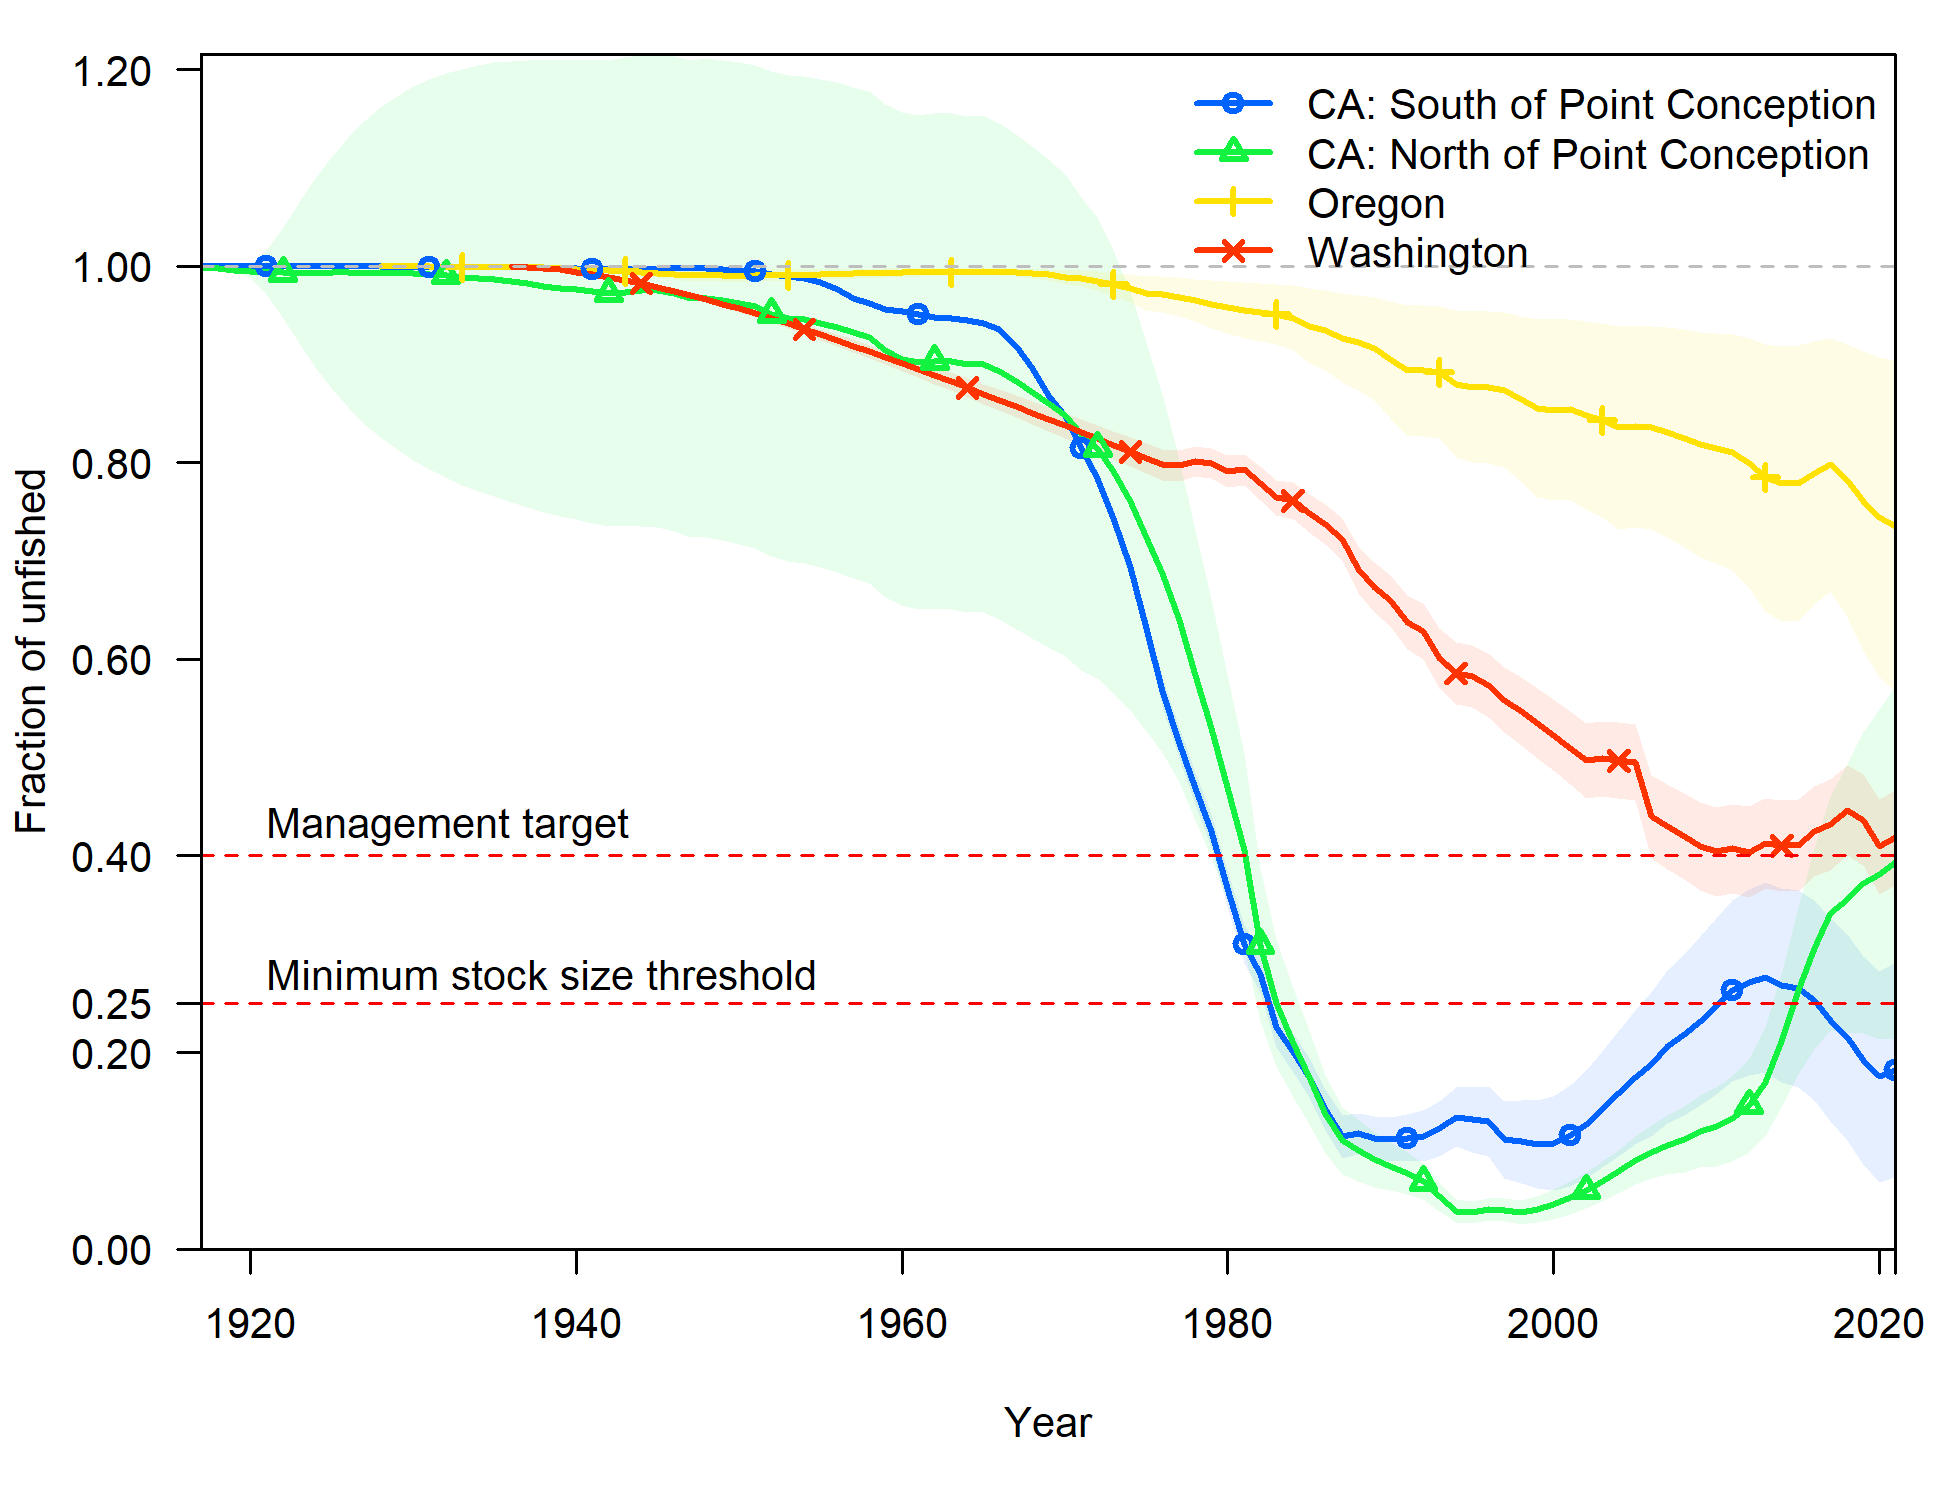
\includegraphics[width=1\textwidth,height=1\textheight]{comprare_compare4_Bratio_uncertainty.png}
\caption{Estimate relative spawning output by assessed area.\label{fig:relb-comparison}}
\end{figure}

\tagmcend\tagstructend

\clearpage

\tagstructbegin{tag=P}\tagmcbegin{tag=P}

\emph{Evidence for Alternative Management Scale}

\leavevmode\tagmcend\tagstructend\par

\tagstructbegin{tag=P}\tagmcbegin{tag=P}

The areas of true population variation in relative stock size may not align with the assessment boundaries as currently defined. State based management is likely not the only factor impacting relative stock sizes across the coast where movement and recruitment patterns likely also influence potential differences in relative stock size.

\leavevmode\tagmcend\tagstructend\par

\tagstructbegin{tag=P}\tagmcbegin{tag=P}

Cope and Punt {\tagstructbegin{tag=Reference}\tagmcbegin{tag=Reference}(2013)\leavevmode\tagmcend\tagstructend}: Conventional stock assessments failed to estimate differing spatial patterns and exploitation (localized depletion) but adequately estimated the overall stock status.

\leavevmode\tagmcend\tagstructend\par

\tagstructbegin{tag=H3}\tagmcbegin{tag=H3}

\hypertarget{size-and-age-composition}{%
\subsubsection{Size and Age Composition}\label{size-and-age-composition}}

\leavevmode\tagmcend\tagstructend

\tagstructbegin{tag=P}\tagmcbegin{tag=P}

\emph{Evidence for Managing at Assessment Scale}

\leavevmode\tagmcend\tagstructend\par

\tagstructbegin{tag=P}\tagmcbegin{tag=P}

Distinct selectivity curves estimated between the recreational and commercial fisheries north and south of Point Conception. While to a lesser degree, the selectivity in Oregon and Washington commercial and recreation fleets also varied from selectivity estimated in other areas.

\leavevmode\tagmcend\tagstructend\par

\tagstructbegin{tag=P}\tagmcbegin{tag=P}

Bosely et al. {\tagstructbegin{tag=Reference}\tagmcbegin{tag=Reference}(2019)\leavevmode\tagmcend\tagstructend}: Specifying the correct form spatial population structure may not e as critical as understanding movement patterns and spatial heterogeneity in fishery selectivity and life-history variation when developing reference points for management.

\leavevmode\tagmcend\tagstructend\par

\tagstructbegin{tag=P}\tagmcbegin{tag=P}

Berger et al. {\tagstructbegin{tag=Reference}\tagmcbegin{tag=Reference}(2021)\leavevmode\tagmcend\tagstructend}: Aligning management assessment areas with with underlying population structure and processes is important, especially when fishing mortality is disproportionate to vulnerable biomass among management areas, demographic parameters (growth and maturity) are not homogeneous within management areas, and connectivity (via recruitment or movement) unknowingly exists among management areas. Bias and risk were greater for assessments that incorrectly span multiple population segments compared to assessments that cover a subset of a population segment, and these results were exacerbated when there was connectivity between population segments. Caveat: The variation is growth and connectivity between areas via recruitment for copper rockfish off the West Coast is currently unknown or uncertain.

\leavevmode\tagmcend\tagstructend\par

\tagstructbegin{tag=P}\tagmcbegin{tag=P}

\emph{Caveat}

\leavevmode\tagmcend\tagstructend\par

\tagstructbegin{tag=P}\tagmcbegin{tag=P}

Rather than creating separate assessments to account for variation in exploitation or life-history variation across areas a more integrated approach could be to apply a spatial assessment that can provide both area- and coastwide population estimates. However, spatial assessments come at the cost of a larger number of parameters to estimate, but general guidance around the key decisions exists when moving to spatial assessments (Punt {\tagstructbegin{tag=Reference}\tagmcbegin{tag=Reference}(2019)\leavevmode\tagmcend\tagstructend}). This approach should be evaluated to understand the trade-offs between adding parameters that may be poorly informed (e.g., movement, recruitment by area) via a spatial assessment approach versus either conducting separate assessments or applying the ``fleets-as-areas'' approach.

\leavevmode\tagmcend\tagstructend\par

\clearpage

\tagstructbegin{tag=H1}\tagmcbegin{tag=H1}

\hypertarget{summary-of-california-stocks}{%
\section{Summary of California stocks}\label{summary-of-california-stocks}}

\leavevmode\tagmcend\tagstructend

\tagstructbegin{tag=P}\tagmcbegin{tag=P}

The 2021 assessment of Copper rockfish off the coast of California assessed as two separate sub-stocks split at Point Conception. The spawning output by area and summed across California along with the relative spawning outputs for each area are provided in Table \ref{tab:ca-ssb}.

\leavevmode\tagmcend\tagstructend\par

\begingroup\fontsize{10}{12}\selectfont
\begingroup\fontsize{10}{12}\selectfont

\tagstructbegin{tag=Table}\tagmcbegin{tag=Table}
\begin{longtable}[t]{l>{\raggedright\arraybackslash}p{1.57cm}>{\raggedright\arraybackslash}p{1.57cm}>{\raggedright\arraybackslash}p{1.57cm}>{\raggedright\arraybackslash}p{1.57cm}>{\raggedright\arraybackslash}p{1.57cm}>{\raggedright\arraybackslash}p{1.57cm}}
\caption{\label{tab:ca-ssb}Spawning output (SO) south and north of Point Conception in California, total spawning output across California, relative spawning output (Rel. SO) north and south of Point Conception, and relative spawning output across California.}\\
\toprule
Year & SO-North & SO-South & SO-CA & Rel. SO-North & Rel. SO-South & Rel. SO-CA\\
\midrule
\endfirsthead
\caption[]{\label{tab:ca-ssb}Spawning output (SO) south and north of Point Conception in California, total spawning output across California, relative spawning output (Rel. SO) north and south of Point Conception, and relative spawning output across California. \textit{(continued)}}\\
\toprule
Year & SO-North & SO-South & SO-CA & Rel. SO-North & Rel. SO-South & Rel. SO-CA\\
\midrule
\endhead

\endfoot
\bottomrule
\endlastfoot
1914 & 415.81 & 233.04 & 648.86 & 1.000 & 1.000 & 1.000\\
1915 & 415.81 & 233.04 & 648.86 & 1.000 & 1.000 & 1.000\\
1916 & 415.81 & 233.04 & 648.86 & 1.000 & 1.000 & 1.000\\
1917 & 415.38 & 233.03 & 648.41 & 0.999 & 1.000 & 0.999\\
1918 & 414.73 & 233.00 & 647.74 & 0.997 & 1.000 & 0.998\\
1919 & 413.98 & 232.98 & 646.97 & 0.996 & 1.000 & 0.997\\
1920 & 413.57 & 232.97 & 646.54 & 0.995 & 1.000 & 0.996\\
1921 & 413.20 & 232.96 & 646.16 & 0.994 & 1.000 & 0.996\\
1922 & 412.99 & 232.95 & 645.94 & 0.993 & 1.000 & 0.996\\
1923 & 412.91 & 232.94 & 645.85 & 0.993 & 1.000 & 0.995\\
1924 & 412.85 & 232.93 & 645.78 & 0.993 & 1.000 & 0.995\\
1925 & 412.97 & 232.92 & 645.89 & 0.993 & 0.999 & 0.995\\
1926 & 412.98 & 232.90 & 645.88 & 0.993 & 0.999 & 0.995\\
1927 & 412.90 & 232.88 & 645.78 & 0.993 & 0.999 & 0.995\\
1928 & 412.99 & 232.86 & 645.86 & 0.993 & 0.999 & 0.995\\
1929 & 412.94 & 232.85 & 645.79 & 0.993 & 0.999 & 0.995\\
1930 & 412.80 & 232.83 & 645.63 & 0.993 & 0.999 & 0.995\\
1931 & 412.38 & 232.81 & 645.20 & 0.992 & 0.999 & 0.994\\
1932 & 411.77 & 232.79 & 644.57 & 0.990 & 0.999 & 0.993\\
1933 & 411.15 & 232.77 & 643.92 & 0.989 & 0.999 & 0.992\\
1934 & 410.55 & 232.76 & 643.31 & 0.987 & 0.999 & 0.991\\
1935 & 410.02 & 232.74 & 642.76 & 0.986 & 0.999 & 0.991\\
1936 & 409.20 & 232.68 & 641.88 & 0.984 & 0.998 & 0.989\\
1937 & 408.38 & 232.65 & 641.02 & 0.982 & 0.998 & 0.988\\
1938 & 407.35 & 232.52 & 639.88 & 0.980 & 0.998 & 0.986\\
1939 & 406.51 & 232.46 & 638.97 & 0.978 & 0.998 & 0.985\\
1940 & 405.99 & 232.42 & 638.41 & 0.976 & 0.997 & 0.984\\
1941 & 405.06 & 232.38 & 637.44 & 0.974 & 0.997 & 0.982\\
1942 & 404.32 & 232.35 & 636.67 & 0.972 & 0.997 & 0.981\\
1943 & 404.83 & 232.36 & 637.19 & 0.974 & 0.997 & 0.982\\
1944 & 405.35 & 232.37 & 637.72 & 0.975 & 0.997 & 0.983\\
1945 & 405.50 & 232.40 & 637.89 & 0.975 & 0.997 & 0.983\\
1946 & 404.16 & 232.42 & 636.58 & 0.972 & 0.997 & 0.981\\
1947 & 402.10 & 232.44 & 634.53 & 0.967 & 0.997 & 0.978\\
1948 & 402.37 & 232.39 & 634.76 & 0.968 & 0.997 & 0.978\\
1949 & 401.30 & 232.24 & 633.54 & 0.965 & 0.997 & 0.976\\
1950 & 400.14 & 232.01 & 632.15 & 0.962 & 0.996 & 0.974\\
1951 & 398.57 & 231.68 & 630.25 & 0.959 & 0.994 & 0.971\\
1952 & 395.58 & 231.04 & 626.62 & 0.951 & 0.991 & 0.966\\
1953 & 393.78 & 230.55 & 624.34 & 0.947 & 0.989 & 0.962\\
1954 & 393.19 & 230.11 & 623.30 & 0.946 & 0.987 & 0.961\\
1955 & 391.72 & 229.22 & 620.94 & 0.942 & 0.984 & 0.957\\
1956 & 389.95 & 227.43 & 617.38 & 0.938 & 0.976 & 0.951\\
1957 & 387.63 & 225.39 & 613.02 & 0.932 & 0.967 & 0.945\\
1958 & 385.83 & 224.09 & 609.92 & 0.928 & 0.962 & 0.940\\
1959 & 379.98 & 222.85 & 602.83 & 0.914 & 0.956 & 0.929\\
1960 & 376.56 & 222.23 & 598.79 & 0.906 & 0.954 & 0.923\\
1961 & 374.91 & 221.65 & 596.57 & 0.902 & 0.951 & 0.919\\
1962 & 375.64 & 220.89 & 596.52 & 0.903 & 0.948 & 0.919\\
1963 & 375.56 & 220.53 & 596.09 & 0.903 & 0.946 & 0.919\\
1964 & 374.29 & 220.21 & 594.50 & 0.900 & 0.945 & 0.916\\
1965 & 374.38 & 219.45 & 593.83 & 0.900 & 0.942 & 0.915\\
1966 & 371.29 & 218.10 & 589.39 & 0.893 & 0.936 & 0.908\\
1967 & 366.95 & 213.92 & 580.87 & 0.882 & 0.918 & 0.895\\
1968 & 362.38 & 208.73 & 571.11 & 0.872 & 0.896 & 0.880\\
1969 & 357.66 & 202.44 & 560.10 & 0.860 & 0.869 & 0.863\\
1970 & 352.64 & 197.30 & 549.94 & 0.848 & 0.847 & 0.848\\
1971 & 344.71 & 189.91 & 534.62 & 0.829 & 0.815 & 0.824\\
1972 & 338.84 & 182.81 & 521.65 & 0.815 & 0.784 & 0.804\\
1973 & 328.96 & 173.21 & 502.17 & 0.791 & 0.743 & 0.774\\
1974 & 316.36 & 161.58 & 477.94 & 0.761 & 0.693 & 0.737\\
1975 & 301.24 & 147.14 & 448.38 & 0.724 & 0.631 & 0.691\\
1976 & 285.72 & 132.18 & 417.90 & 0.687 & 0.567 & 0.644\\
1977 & 265.76 & 119.95 & 385.70 & 0.639 & 0.515 & 0.594\\
1978 & 242.71 & 109.12 & 351.84 & 0.584 & 0.468 & 0.542\\
1979 & 220.21 & 99.11 & 319.32 & 0.530 & 0.425 & 0.492\\
1980 & 195.23 & 85.44 & 280.68 & 0.470 & 0.367 & 0.433\\
1981 & 168.51 & 72.17 & 240.68 & 0.405 & 0.310 & 0.371\\
1982 & 128.65 & 65.18 & 193.83 & 0.309 & 0.280 & 0.299\\
1983 & 104.02 & 52.56 & 156.58 & 0.250 & 0.226 & 0.241\\
1984 & 87.13 & 46.53 & 133.66 & 0.210 & 0.200 & 0.206\\
1985 & 72.65 & 40.60 & 113.25 & 0.175 & 0.174 & 0.175\\
1986 & 56.82 & 33.06 & 89.88 & 0.137 & 0.142 & 0.139\\
1987 & 45.88 & 26.58 & 72.46 & 0.110 & 0.114 & 0.112\\
1988 & 41.70 & 27.31 & 69.01 & 0.100 & 0.117 & 0.106\\
1989 & 37.85 & 26.31 & 64.15 & 0.091 & 0.113 & 0.099\\
1990 & 34.82 & 25.95 & 60.77 & 0.084 & 0.111 & 0.094\\
1991 & 32.15 & 26.30 & 58.45 & 0.077 & 0.113 & 0.090\\
1992 & 28.39 & 26.79 & 55.18 & 0.068 & 0.115 & 0.085\\
1993 & 22.16 & 28.53 & 50.69 & 0.053 & 0.122 & 0.078\\
1994 & 16.05 & 31.21 & 47.26 & 0.039 & 0.134 & 0.073\\
1995 & 15.60 & 30.65 & 46.25 & 0.038 & 0.132 & 0.071\\
1996 & 16.79 & 30.29 & 47.08 & 0.040 & 0.130 & 0.073\\
1997 & 16.41 & 25.95 & 42.37 & 0.039 & 0.111 & 0.065\\
1998 & 15.44 & 25.45 & 40.89 & 0.037 & 0.109 & 0.063\\
1999 & 16.75 & 24.76 & 41.51 & 0.040 & 0.106 & 0.064\\
2000 & 18.93 & 24.98 & 43.90 & 0.046 & 0.107 & 0.068\\
2001 & 21.74 & 26.83 & 48.57 & 0.052 & 0.115 & 0.075\\
2002 & 24.84 & 29.53 & 54.38 & 0.060 & 0.127 & 0.084\\
2003 & 28.64 & 33.08 & 61.72 & 0.069 & 0.142 & 0.095\\
2004 & 32.70 & 36.82 & 69.52 & 0.079 & 0.158 & 0.107\\
2005 & 37.57 & 40.76 & 78.33 & 0.090 & 0.175 & 0.121\\
2006 & 41.04 & 43.68 & 84.72 & 0.099 & 0.187 & 0.131\\
2007 & 44.00 & 47.92 & 91.92 & 0.106 & 0.206 & 0.142\\
2008 & 46.33 & 50.77 & 97.10 & 0.111 & 0.218 & 0.150\\
2009 & 49.58 & 54.01 & 103.59 & 0.119 & 0.232 & 0.160\\
2010 & 51.80 & 57.50 & 109.30 & 0.125 & 0.247 & 0.168\\
2011 & 55.04 & 61.25 & 116.29 & 0.132 & 0.263 & 0.179\\
2012 & 60.66 & 63.22 & 123.88 & 0.146 & 0.271 & 0.191\\
2013 & 70.63 & 64.35 & 134.98 & 0.170 & 0.276 & 0.208\\
2014 & 88.01 & 62.52 & 150.53 & 0.212 & 0.268 & 0.232\\
2015 & 109.29 & 61.70 & 170.99 & 0.263 & 0.265 & 0.264\\
2016 & 127.02 & 58.89 & 185.91 & 0.305 & 0.253 & 0.287\\
2017 & 141.90 & 54.21 & 196.11 & 0.341 & 0.233 & 0.302\\
2018 & 147.97 & 50.17 & 198.14 & 0.356 & 0.215 & 0.305\\
2019 & 154.78 & 44.70 & 199.48 & 0.372 & 0.192 & 0.307\\
2020 & 158.56 & 40.81 & 199.37 & 0.381 & 0.175 & 0.307\\
2021 & 163.51 & 42.28 & 205.79 & 0.393 & 0.181 & 0.317\\*
\end{longtable}
\leavevmode\tagmcend\tagstructend\par
\endgroup{}
\endgroup{}

\tagstructbegin{tag=H1}\tagmcbegin{tag=H1}

\hypertarget{proposed-allocation-of-yield-among-federal-management-areas}{%
\section{Proposed Allocation of Yield Among Federal Management Areas}\label{proposed-allocation-of-yield-among-federal-management-areas}}

\leavevmode\tagmcend\tagstructend

\tagstructbegin{tag=P}\tagmcbegin{tag=P}

The 2021 northern California base model for copper rockfish represents U.S. waters between 34{\tagstructbegin{tag=Formula}\tagmcbegin{tag=Formula}\(^\circ\)\leavevmode\tagmcend\tagstructend} 27' N. lat. and the California-Oregon border 42{\tagstructbegin{tag=Formula}\tagmcbegin{tag=Formula}\(^\circ\)\leavevmode\tagmcend\tagstructend} 00' N. lat. Federal management of the nearshore rockfish complex, that includes copper rockfish, is based on areas north and south of 40{\tagstructbegin{tag=Formula}\tagmcbegin{tag=Formula}\(^\circ\)\leavevmode\tagmcend\tagstructend} 10' N. lat. Therefore, yield estimates from the California base model must be divided between the norther and southern management areas in order to determine the contribution of copper rockfish to the nearshore rockfish overfishing limit (OFL).

\leavevmode\tagmcend\tagstructend\par

\tagstructbegin{tag=P}\tagmcbegin{tag=P}

Ideally, allocation by area would be based on calculations of habitat by area and/or estimates of biomass by area. Unfortunately neither of these estimates were available for copper rockfish to inform allocations by area. In lieu of this information, historical catches by each region were used to recommend allocation percents by area. Total removals from the recreational and commercial fleets between 2005 - 2020 by areas north and south of 40{\tagstructbegin{tag=Formula}\tagmcbegin{tag=Formula}\(^\circ\)\leavevmode\tagmcend\tagstructend} 10' N. lat. were calculated. During this period a total of 3.9 percent of all removals were from areas north of 40{\tagstructbegin{tag=Formula}\tagmcbegin{tag=Formula}\(^\circ\)\leavevmode\tagmcend\tagstructend} 10' N. lat. Based on this the recommend allocations of the OFLs from the northern California model 3.9 percent should be allocated to the north nearshore rockfish complex with 96.1 percent to the southern complex.

\leavevmode\tagmcend\tagstructend\par

\clearpage

\tagstructbegin{tag=H1}\tagmcbegin{tag=H1}

\hypertarget{references}{%
\section{References}\label{references}}

\leavevmode\tagmcend\tagstructend

\tagstructbegin{tag=BibEntry}\tagmcbegin{tag=BibEntry}

\hypertarget{refs}{}
\begin{CSLReferences}{1}{0}
\leavevmode\hypertarget{ref-berger_incoherent_2021}{}%
Berger, Aaron M, Jonathan J Deroba, Katelyn M Bosley, Daniel R Goethel, Brian J Langseth, Amy M Schueller, and Dana H Hanselman. 2021. {``Incoherent Dimensionality in Fisheries Management: Consequences of Misaligned Stock Assessment and Population Boundaries.''} Edited by Valerio Bartolino. \emph{ICES Journal of Marine Science} 78 (1): 155--71. \url{https://doi.org/10.1093/icesjms/fsaa203}.

\leavevmode\hypertarget{ref-bosley_overcoming_2019}{}%
Bosley, Katelyn M., Daniel R. Goethel, Aaron M. Berger, Jonathan J. Deroba, Kari H. Fenske, Dana H. Hanselman, Brian J. Langseth, and Amy M. Schueller. 2019. {``Overcoming Challenges of Harvest Quota Allocation in Spatially Structured Populations.''} \emph{Fisheries Research} 220 (December): 105344. \url{https://doi.org/10.1016/j.fishres.2019.105344}.

\leavevmode\hypertarget{ref-buonaccorsi_molecular_2004}{}%
Buonaccorsi, V. P., M. Westerman, J. Stannard, C. Kimbrell, E. Lynn, and R. D. Vetter. 2004. {``Molecular Genetic Structure Suggests Limited Larval Dispersal in Grass Rockfish, {Sebastes} Rastrelliger.''} \emph{Marine Biology} -1 (1): 1--1. \url{https://doi.org/10.1007/s00227-004-1362-2}.

\leavevmode\hypertarget{ref-buonaccorsi_population_2002}{}%
Buonaccorsi, Vincent P, Carol A Kimbrell, Eric A Lynn, and Russell D Vetter. 2002. {``Population Structure of Copper Rockfish (\emph{{Sebastes} Caurinus}) Reflects Postglacial Colonization and Contemporary Patterns of Larval Dispersal.''} \emph{Canadian Journal of Fisheries and Aquatic Sciences} 59 (8): 1374--84. \url{https://doi.org/10.1139/f02-101}.

\leavevmode\hypertarget{ref-cope_data-moderate_2013}{}%
Cope, Jason, E. J. Dick, Alec MacCall, Melissa Monk, Braden Soper, and Chantel Wetzel. 2013. {``Data-Moderate Stock Assessments for Brown, {China}, Copper, Sharpchin, Stripetail, and Yellowtail Rockfishes and {English} and Rex Soles in 2013.''} 7700 Ambassador Place NE, Suite 200, Portland, OR: Pacific Fishery Management Council. \url{http://www.academia.edu/download/44999856/CopeetalDataModerate2013.pdf}.

\leavevmode\hypertarget{ref-field_spatiotemporal_2021}{}%
Field, John C., Rebecca R. Miller, Jarrod A. Santora, Nick Tolimieri, Melissa A. Haltuch, Richard D. Brodeur, Toby D. Auth, et al. 2021. {``Spatiotemporal Patterns of Variability in the Abundance and Distribution of Winter-Spawned Pelagic Juvenile Rockfish in the {California} {Current}.''} Edited by Geir Ottersen. \emph{PLOS ONE} 16 (5): e0251638. \url{https://doi.org/10.1371/journal.pone.0251638}.

\leavevmode\hypertarget{ref-gertseva_spatial_2017}{}%
Gertseva, Vladlena, Sean E. Matson, and Jason Cope. 2017. {``Spatial Growth Variability in Marine Fish: Example from {Northeast} {Pacific} Groundfish.''} Edited by Emory Anderson. \emph{ICES Journal of Marine Science} 74 (6): 1602--13. \url{https://doi.org/10.1093/icesjms/fsx016}.

\leavevmode\hypertarget{ref-hannah_length_2014}{}%
Hannah, Robert W. 2014. {``Length and Age at Maturity of Female Copper Rockfish (\emph{{Sebastes} Caurinus}) from {Oregon} Waters Based on Histological Evaluation of Ovaries.''} Information Reports 2014-04. Oregon Department of Fish; Wildlife.

\leavevmode\hypertarget{ref-johansson_influence_2008}{}%
Johansson, M. L., M. A. Banks, K. D. Glunt, H. M. Hassel-Finnegan, and V. P. Buonaccorsi. 2008. {``Influence of Habitat Discontinuity, Geographical Distance, and Oceanography on Fine-Scale Population Genetic Structure of Copper Rockfish ( \emph{{Sebastes} Caurinus} ).''} \emph{Molecular Ecology} 17 (13): 3051--61. \url{https://doi.org/10.1111/j.1365-294X.2008.03814.x}.

\leavevmode\hypertarget{ref-keller_canary_2018}{}%
Keller, Aa, Ph Frey, Jr Wallace, Ma Head, Cr Wetzel, Jm Cope, and Jh Harms. 2018. {``Canary Rockfishes {Sebastes} Pinniger Return from the Brink: Catch, Distribution and Life History Along the {US} West Coast ({Washington} to {California}).''} \emph{Marine Ecology Progress Series} 599 (July): 181--200. \url{https://doi.org/10.3354/meps12603}.

\leavevmode\hypertarget{ref-keller_variation_2012}{}%
Keller, Aimee A., Kyle J. Molton, Allan C. Hicks, Melissa Haltuch, and Chantell Wetzel. 2012. {``Variation in Age and Growth of Greenstriped Rockfish ({Sebastes} Elongatus) Along the {U}.{S}. West Coast ({Washington} to {California}).''} \emph{Fisheries Research} 119-120 (May): 80--88. \url{https://doi.org/10.1016/j.fishres.2011.12.012}.

\leavevmode\hypertarget{ref-lea_biological_1999}{}%
Lea, Robert N, Robert D McAllister, and David A VenTresca. 1999. {``Biological Sspects of Nearshore Rockfishes of the Genus Sebastes from {Central} {California} with Notes on Ecologically Related Sport Fishes.''} Fish Bulletin 177. State of California The Resources Agency Department of Fish; Game.

\leavevmode\hypertarget{ref-lowe_site_2009}{}%
Lowe, Christopher G., Kim M. Anthony, Erica T. Jarvis, Lyall F. Bellquist, and Milton S. Love. 2009. {``Site {Fidelity} and {Movement} {Patterns} of {Groundfish} {Associated} with {Offshore} {Petroleum} {Platforms} in the {Santa} {Barbara} {Channel}.''} \emph{Marine and Coastal Fisheries} 1 (1): 71--89. \url{https://doi.org/10.1577/C08-047.1}.

\leavevmode\hypertarget{ref-markel_rockfish_2011}{}%
Markel, Russell Wayne. 2011. {``Rockfish Recruitment and Trophic Dynamics on the West Coast of Vancouver Island: Fishing, Ocean, Climate, and Sea Otters.''} \emph{Dissertation, University of British Columbia}, 146.

\leavevmode\hypertarget{ref-mcgilliard_accounting_2015}{}%
McGilliard, Carey R., André E. Punt, Richard D. Methot, and Ray Hilborn. 2015. {``Accounting for Marine Reserves Using Spatial Stock Assessments.''} Edited by Larry Jacobson. \emph{Canadian Journal of Fisheries and Aquatic Sciences} 72 (2): 262--80. \url{https://doi.org/10.1139/cjfas-2013-0364}.

\leavevmode\hypertarget{ref-punt_which_2015}{}%
Punt, André E., Malcolm Haddon, and Geoffrey N. Tuck. 2015. {``Which Assessment Configurations Perform Best in the Face of Spatial Heterogeneity in Fishing Mortality, Growth and Recruitment? {A} Case Study Based on Pink Ling in {Australia}.''} \emph{Fisheries Research} 168 (August): 85--99. \url{https://doi.org/10.1016/j.fishres.2015.04.002}.

\leavevmode\hypertarget{ref-punt_spatial_2019}{}%
Punt, André E. 2019. {``Spatial Stock Assessment Methods: {A} Viewpoint on Current Issues and Assumptions.''} \emph{Fisheries Research} 213 (May): 132--43. \url{https://doi.org/10.1016/j.fishres.2019.01.014}.

\leavevmode\hypertarget{ref-reynolds_application_2010}{}%
Reynolds, Brad F., Sean P. Powers, and Mary Anne Bishop. 2010. {``Application of {Acoustic} {Telemetry} to {Assess} {Residency} and {Movements} of {Rockfish} and {Lingcod} at {Created} and {Natural} {Habitats} in {Prince} {William} {Sound}.''} Edited by Daniel J. Rankin. \emph{PLoS ONE} 5 (8): e12130. \url{https://doi.org/10.1371/journal.pone.0012130}.

\leavevmode\hypertarget{ref-sivasundar_life_2010}{}%
Sivasundar, Arjun, and Stephen R. Palumbi. 2010. {``Life History, Ecology and the Biogeography of Strong Genetic Breaks Among 15 Species of {Pacific} Rockfish, {Sebastes}.''} \emph{Marine Biology} 157 (7): 1433--52. \url{https://doi.org/10.1007/s00227-010-1419-3}.

\leavevmode\hypertarget{ref-tolimieri_home_2009}{}%
Tolimieri, N, K Andrews, G Williams, S Katz, and Ps Levin. 2009. {``Home Range Size and Patterns of Space Use by Lingcod, Copper Rockfish and Quillback Rockfish in Relation to Diel and Tidal Cycles.''} \emph{Marine Ecology Progress Series} 380 (April): 229--43. \url{https://doi.org/10.3354/meps07930}.

\leavevmode\hypertarget{ref-waples_what_2006}{}%
Waples, Robin S., and Oscar Gaggiotti. 2006. {``What Is a Population? {An} Empirical Evaluation of Some Genetic Methods for Identifying the Number of Gene Pools and Their Degree of Connectivity.''} \emph{Molecular Ecology} 15 (6): 1419--39. \url{https://doi.org/10.1111/j.1365-294X.2006.02890.x}.

\leavevmode\hypertarget{ref-ying_risks_2011}{}%
Ying, Yiping, Yong Chen, Longshan Lin, Tianxian Gao, and Terrance Quinn. 2011. {``Risks of Ignoring Fish Population Spatial Structure in Fisheries Management.''} \emph{Canadian Journal of Fisheries and Aquatic Sciences} 68 (12): 2101--20. \url{https://doi.org/10.1139/f2011-116}.

\end{CSLReferences}

\leavevmode\tagmcend\tagstructend
\end{document}
